\section{Problem}
The number of interactive applications increased rapidly since the computational power of personal computers is increasing. There are new technologies like motion sensors and controller to interact with a software. During this development, the number of interactive applications built around sound detection and classification is growing as well. Examples for successful applications are apps which can match recorded music with it's song title and interpret or karaoke games which recognized how good the singer strikes the right notes and texts.

Furthermore, the broadband of the Internet and thus the performance of web-services are still making substantial progress. There are ever new web technologies, which enable the web to become more and more interactive. This also leads to plenty of e-learning websites, which find favor with a large audience. Especially language learning platforms and platforms to playfully support kids by learning the alphabet or some mathematics became quite famous in the past few years.

With my master thesis I follow these trends and add even more interaction to the web. The basis of my work is the online e-learning platform Easydrum. It empowers its users to learn how to play a drum-set online. The platform provides different drum lessons and exercises. An e-drum-set can be connected to do these exercises. During practicing, the website gives feedback on the users performance.

The disadvantage of the platform was, that you have to use an e-drum-set to receive feedback. But teaching drums with a „real“ drum-set is much more effective because playing an e-drum-set feels different and adulterated. Most musicians avoid this kind of drums. Therefore, the aim of this master thesis is to allow the use of a non-electronic drum-set. In order to achieve this I want to develop a software which recognizes and analyzes the sounds of drums and cymbals. The software has to identify if the correct drum or cymbal has been played at the right time. Several drums or cymbals can be played at the same time. The app should run in real-time on the web with the help of the Web Audio API which is documented in \autocite{WebAudioApi:2015}.

\section{Related work}
There had been a lot of researches on similar subjects in the past. Automatic detection and classification of drum sounds has been studied in the context of music information retrieval for numerous purposes, including metrical analysis, database labeling and searches, automatic transcription, and interactive musical systems.

An early work was introduced in 1994 by Goto and Muraoka in \autocite[]{Goto:1994}. Their system concerns drum transcription which was used as a support in an audio-based real-time beat tracking system. M. Goto continued this work and developed an audio-based real-time beat tracking system for music with or without drum-sounds \autocite[]{Goto:2001}. This researches are an important basic for every following work in the field of beat tracking and drum transcription.

A work similar to this approach, by the Aalborg University from 2007 is about the automated recognition of drum types \autocite[]{Christophersen:2007}. Audio files with drum sounds are analyzed and transcribed to a readable format. The resulting algorithm can distinguish between a kick drum, a snare drum and a hi-hat. The algorithm is separated in onset detection, a feature vector and classification. The significant distinction to my master thesis is, that their system does not support real-time. Thus, the onset detection part of the papers algorithm does not work in my case, but the feature vector and the classification part were a good inspiration for my work. Another difference is, that in my research there is a configuration of the used drum kit in the beginning, which makes it much easier and faster to recognize the played drums.

For the real-time part of my algorithm, I considered a paper published in 2010, which deals with real-time automatic detection and labeling of percussive sounds for interactive systems \autocite[]{Simsekli:2011}. In this paper, a model-based algorithm for detection of percussive events and test the algorithm on the detection and classification of different percussive sounds is introduced. The model is trained offline on different percussive sounds using the expectation maximization approach for learning spectral templates for each sound and is able to run online to detect and classify sounds from audio stream input by a Hidden Markov Model.

Based on these researches I want to implement the functionality of using a non electronic drum-set with Easydrum.

\section{Background and Theory}

\subsection{Introduction}

\subsection{Drum Basics}

\subsubsection{Drum set}

\subsubsection{Notation}

\subsection{Easydrum}

\subsection{Previous Research}

\subsubsection{Musical signals}

%figure 1 Bello:2005
\begin{figure}[h]
	\centering
	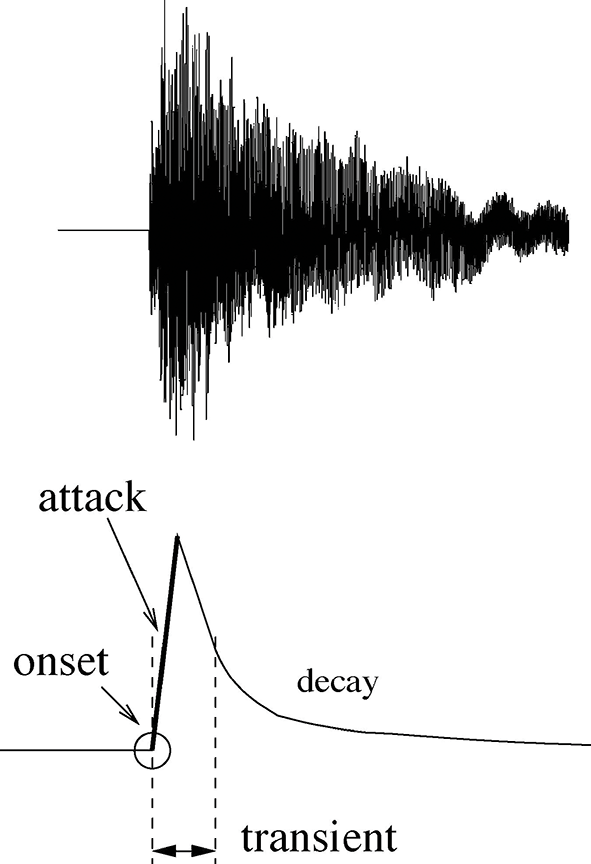
\includegraphics{images/bello_2005_Seite_01_Bild_0001.jpg}
	\label{}
	%for reference to this figure
	\caption{`Attack', `transient', `decay', and `onset' in the ideal case of a single note \autocite[Fig. 1]{Bello:2005}.}
	\label{fig:MusicalSignal}
\end{figure}

The gradient of a musical signal can be described by tree terms which name a certain period or a point in time. These are the transient, the attack and the onset \ref{fig:MusicalSignal}.

The significant the signal is the transient. It describes the time interval, where the musical signal evolves quickly in some nontrivial or relatively unpredictable way. In the case of a drum sound it is the moment when the stick hits the drum. In \autocite[]{Bello:2005} it is assumed that the human ear cannot distinguish between two transients less than 10 ms apart. After the transient, the sound decays. The attack is the part of the transient during which the amplitude of the sound increases. The onset is usually the first identifiable point in time where the transient or attack can be detected.

For my software I will need an algorithm which detects the offset of any played drum in real-time. Furthermore, the appendant transient need to be analyzed for the classification of the played drum.

\subsubsection{Onset Detection}

%figure 2 Bello:2005
\begin{figure}[h]
	\centering
	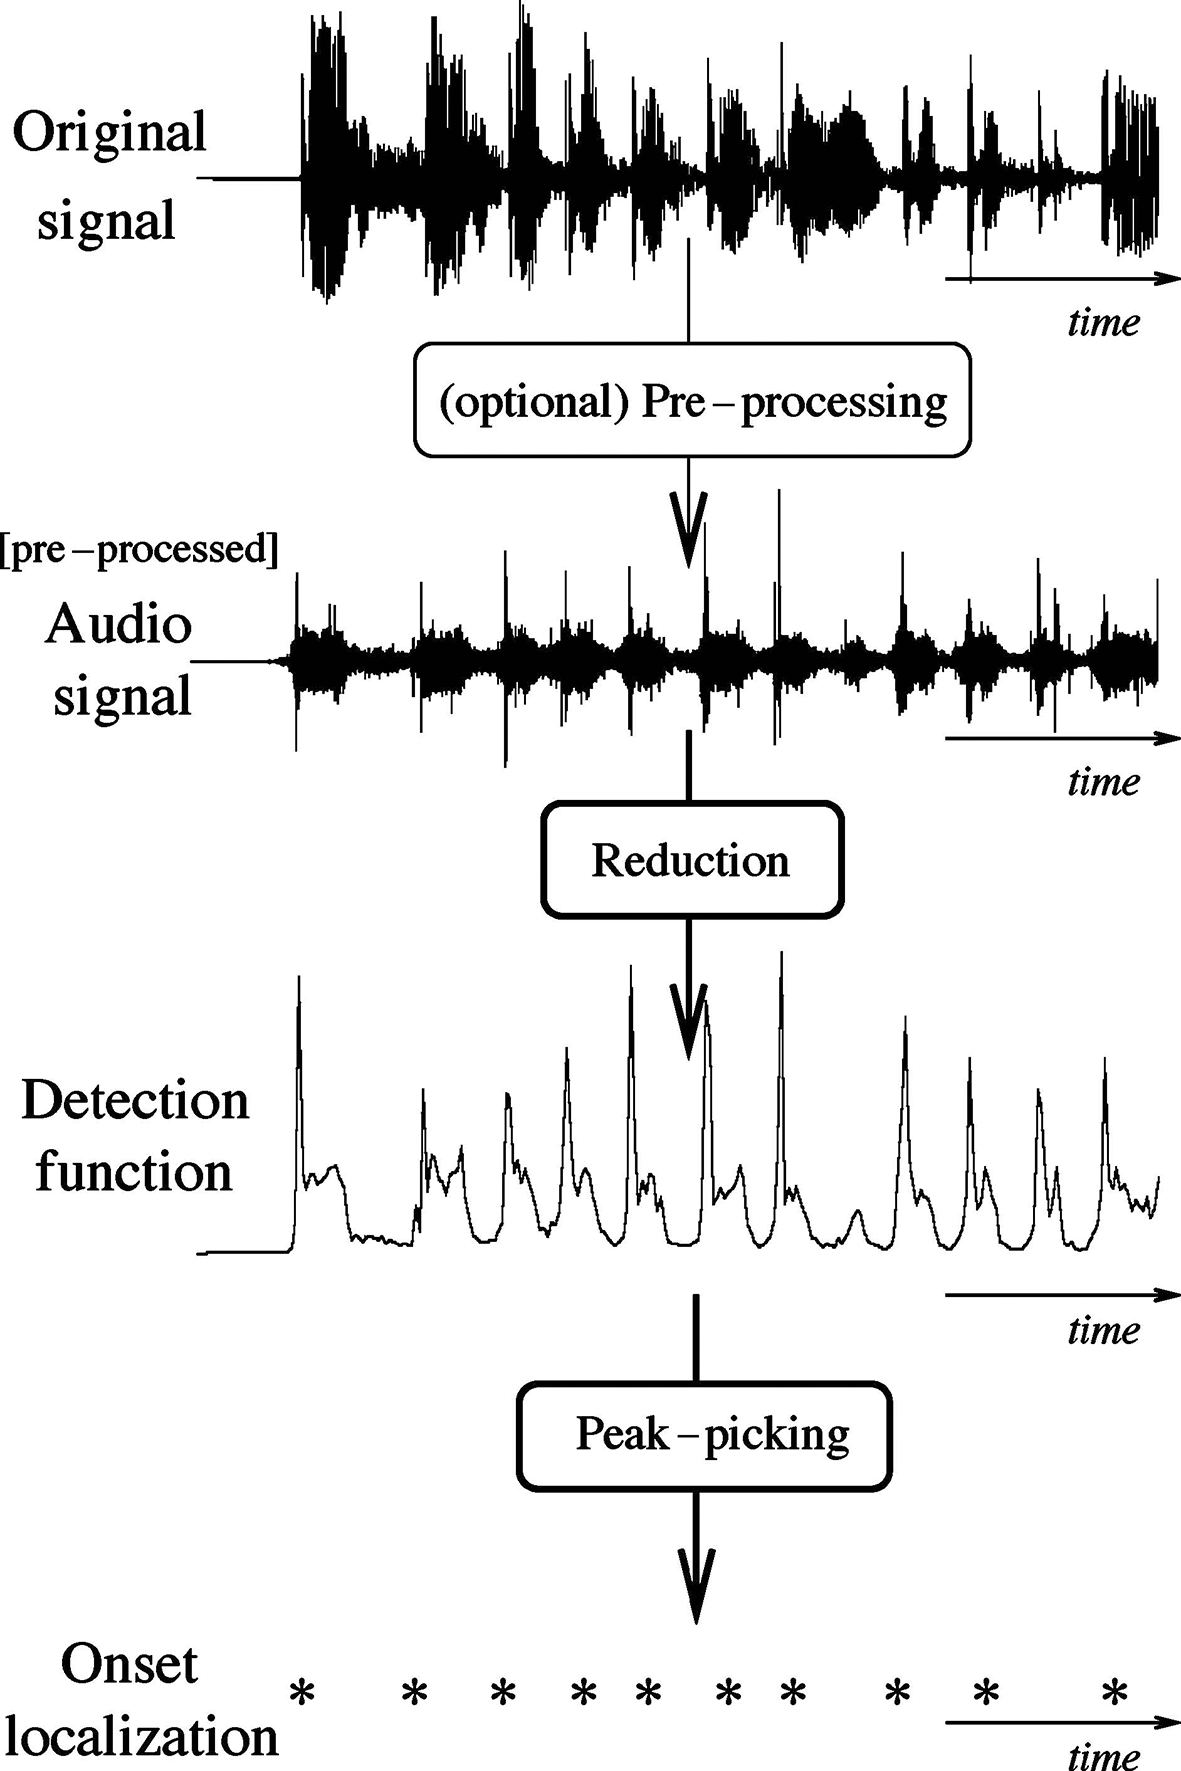
\includegraphics{images/bello_2005_Seite_02_Bild_0001.jpg}
	\label{}
	%for reference to this figure
	\caption{Flowchart of a standard onset detection algorithm \autocite[Fig. 2]{Bello:2005}.}
	\label{fig:StandardOnsetDetection}
\end{figure}

Onset Detection will be an important part of this work. It detects if a new drum is beaten.
There are many different methods of Onset Detection right now. \autocite[]{Bello:2005} describes some important ones. The paper explains methods based on a signal's amplitude envelope, spectral magnitudes and phases, time-frequency representation and methods based on probabilistic signal models. It focuses on note onset detection in musical signals.


\section{Methods}

\subsection{Drumset}
% Description and Pictures of Test Drumset

% Explain 3 kinds of Diagramms 
% peakdetection
% Show Examples
\subsubsection{Single Drums}
\subsubsubsection{Bassdrum}

\subsection{Onset Detection}

\subsection{Feature Extraction}
\subsubsection{Peaks in Frequency Spectrum}
\subsubsection{Root Mean Square Energy}
\subsubsection{Phase Shift and Steadiness}

\subsection{Training System}

\subsection{Real-Time Analysis}

\subsection{Integration in Easydrum}

\section{Conclusion}
\subsection{Summary}
\subsection{Future Research}